\documentclass[a4paper, 12pt, finnish]{article}
\usepackage{babel}
\usepackage[utf8]{inputenc}
\usepackage[T1]{fontenc}
\usepackage{amsmath}
\usepackage{geometry}
\geometry{a4paper}
\usepackage{graphicx}
\usepackage{float}
\usepackage{wrapfig}
\usepackage{caption}
\usepackage{eurosym}
\usepackage[section]{placeins}
\usepackage{url}
\usepackage[hidelinks]{hyperref}
\usepackage{hyperref}
\usepackage{subcaption}
\usepackage{lipsum}
\usepackage[table,xcdraw]{xcolor}
\renewcommand{\figurename}{Kaavio }
\addto\captionsfinnish{\renewcommand{\figurename}{Kaavio}}
\def\UrlBreaks{\do\/\do-} %% Line breakit urleissa
\graphicspath{{Pictures/}} % Kuvien lähde
\begin{document}
\title{MX Linux 18 käyttöönotto, käyttö ja ohjeistus \\ \large Projektisuunnitelma}
\author{Iiro Aarnio\\ Tampereen seudun ammattiopisto}
\maketitle
\thispagestyle{empty}
\newpage
\thispagestyle{empty}
\newpage
\begin{table}[htpb]
\begin{tabular}{llll}
Versiohistoria &            &                         &             \\
\rowcolor[HTML]{FFCCC9}
Versio         & Päivämäärä & Muutosperuste           & Tekijä      \\
1.0              & 4.6.2019   & Ensimmäinen vedos       & Iiro Aarnio \\
\end{tabular}
\end{table}

%\begin{table}[h:wtpb]
%\begin{tabular}{lll}
%Jakelu &            &                                  \\
%\rowcolor[HTML]{FFCCC9}
%Tekijä         & Tulostettu & Jakelu                 \\
%Iiro Aarnio              & Ei ole   & Leena Järvenkylä-Niemi \\
%\end{tabular}
%\end{table}
\newpage
%%%%%%%%%%%%%%%%%%%%%           Table of Contents
\thispagestyle{empty}
\tableofcontents
\newpage
%%%%%%%%%%%%%%%%%%%%%           Table of Contents
\pagenumbering{arabic}
\section{Tehtävä}
Projektin tehtävänä on opiskella MX Linux 18 -GNU/Linux-jakelun käyttö, ja tehdä siitä käyttäjäystävällinen ohjekirja. 

\section{Tulostavoitteet}
Tehtävä on valmis kun on laadittu MX Linux 18 -jakelun käyttöönotosta ja peruskäytöstä tarkka sekä laaja ohjekirja, ja kun päätöspalaveri on pidetty.
\\\\
Laatutavoite: projektin dokumentaatiossa pyritään noudattamaan selvää suomen kieltä.

\section{Rajaukset}
Projektiin eivät kuulu laitteiston käyttöönotto, oheislaitteiden käyttöönotto, laitteistoajureiden opastus, tietoturvaohjeistus eikä asennusmedian luonnin opastus.
\section{Työvaiheet}
Työvaiheita on kuvattu seuraavassa kaaviossa.
\begin{figure}[!htpb]
    \centering
    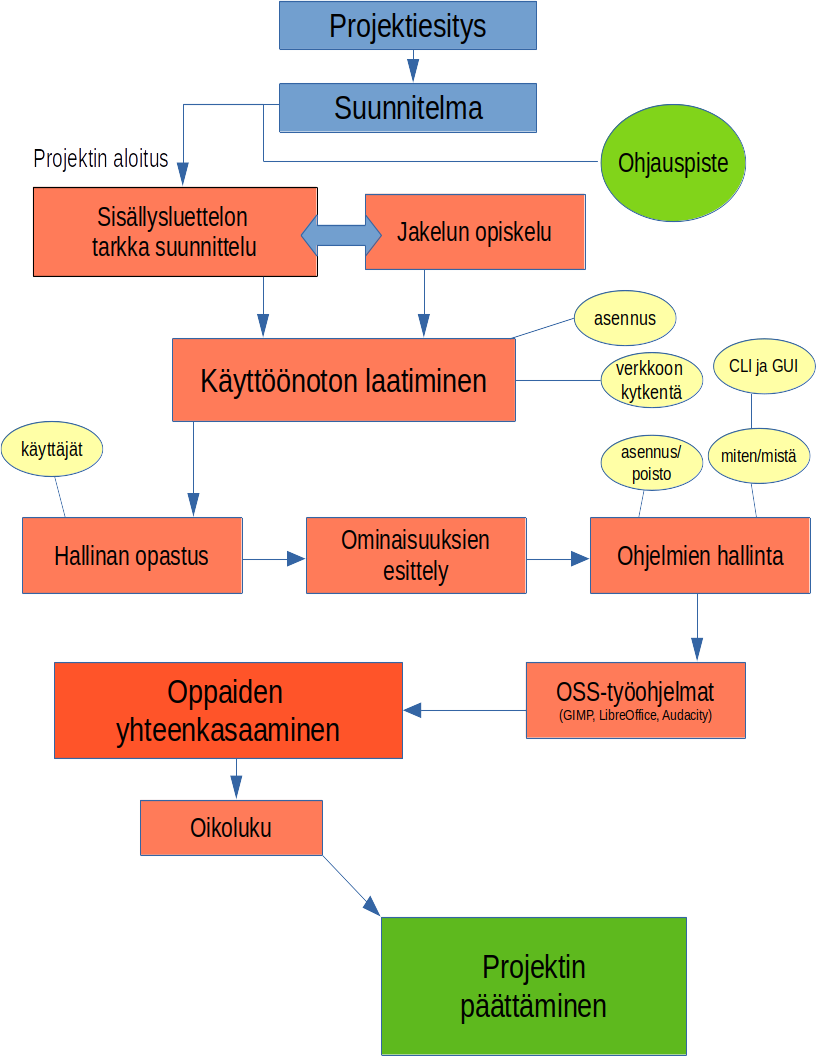
\includegraphics[width=\textwidth]{kaaviokuva}
    \caption{Työvaiheet}
    \label{}
\end{figure}

\end{document}
